
%%\documentclass[12pt,preprint]{aastex}

%% manuscript produces a one-column, double-spaced document:

%% \documentclass[10pt,manuscript]{aastex}

%% preprint2 produces a double-column, single-spaced document:
\documentclass[preprint2,iop,numberedappendix,twocolappendix,appendixfloats]{emulateapj}
%% \documentclass[preprint2,iop]{aastex}

%% \documentclass[preprint2,longabstract]{aastex}

%% \usepackage{ccaption}
%% \captionstyle{\raggedright}
\usepackage[caption=false]{subfig}
\usepackage{amsmath}
\usepackage{footnote}
\usepackage{url}
\bibpunct{(}{)}{;}{a}{}{,} 
\captionsetup{belowskip=12pt,aboveskip=4pt}
\setlength{\textfloatsep}{10pt plus 1.0pt minus 2.0pt}
\newcommand{\dif}{\mathrm{d}}
%% \renewcommand*{\thefootnote}{\fnsymbol{footnote}}

\def\nar{{New~A~Rev.}}          % New Astronomy Review
\def\pasa{{PASA}}               % Publications of the Astron. Soc. of Australia

%% \bibliographystyle{mn2e}
%% \bibliographystyle{apj}

\shorttitle{Effects of Beam Chromaticity in EoR Power Spectra Measurements}
\shortauthors{Thyagarajan et~al.}

\def\ASU{\altaffilmark{1}}
\def\ASUtxt{\altaffiltext{1}{Arizona State University, School of Earth and Space Exploration, Tempe, AZ 85287, USA}}

\def\myemail{\altaffilmark{*}}
\def\myemailtxt{\altaffiltext{*}{e-mail: t\_nithyanandan@asu.edu}}

\def\UW{\altaffilmark{2}}
\def\UWtxt{\altaffiltext{2}{University of Washington, Department of Physics, Seattle, WA 98195, USA}}

\def\SKASA{\altaffilmark{3}}
\def\SKASAtxt{\altaffiltext{3}{Square Kilometre Array South Africa (SKA SA), Park Road, Pinelands 7405, South Africa}}

\def\RU{\altaffilmark{4}}
\def\RUtxt{\altaffiltext{4}{Department of Physics and Electronics, Rhodes University, Grahamstown 6140, South Africa}}

\def\CfA{\altaffilmark{5}}
\def\CfAtxt{\altaffiltext{5}{Harvard-Smithsonian Center for Astrophysics, Cambridge, MA 02138, USA}}

\def\ANU{\altaffilmark{6}}
\def\ANUtxt{\altaffiltext{6}{Australian National University, Research School of Astronomy and Astrophysics, Canberra, ACT 2611, Australia}}

\def\CAASTRO{\altaffilmark{7}}
\def\CAASTROtxt{\altaffiltext{7}{ARC Centre of Excellence for All-sky Astrophysics (CAASTRO)}}

\def\Haystack{\altaffilmark{8}}
\def\Haystacktxt{\altaffiltext{8}{MIT Haystack Observatory, Westford, MA 01886, USA}}

\def\MIT{\altaffilmark{9}}
\def\MITtxt{\altaffiltext{9}{MIT Kavli Institute for Astrophysics and Space Research, Cambridge, MA 02139, USA}}

\def\Curtin{\altaffilmark{10}}
\def\Curtintxt{\altaffiltext{10}{International Centre for Radio Astronomy Research, Curtin University, Perth, WA 6845, Australia}}

\def\Victoria{\altaffilmark{11}}
\def\Victoriatxt{\altaffiltext{11}{Victoria University of Wellington, School of Chemical \& Physical Sciences, Wellington 6140, New Zealand}}

\def\UWisc{\altaffilmark{12}}
\def\UWisctxt{\altaffiltext{12}{University of Wisconsin--Milwaukee, Department of Physics, Milwaukee, WI 53201, USA}}

\def\UMichigan{\altaffilmark{13}}
\def\UMichigantxt{\altaffiltext{13}{University of Michigan, Department of Atmospheric, Oceanic and Space Sciences, Ann Arbor, MI 48109, USA}}

\def\UMelbourne{\altaffilmark{14}}
\def\UMelbournetxt{\altaffiltext{14}{The University of Melbourne, School of Physics, Parkville, VIC 3010, Australia}}

\def\USydney{\altaffilmark{15}}
\def\USydneytxt{\altaffiltext{15}{The University of Sydney, Sydney Institute for Astronomy, School of Physics, NSW 2006, Australia}}

\def\CASS{\altaffilmark{16}}
\def\CASStxt{\altaffiltext{16}{CSIRO Astronomy and Space Science (CASS), PO Box 76, Epping, NSW 1710, Australia}}

\def\Tata{\altaffilmark{17}}
\def\Tatatxt{\altaffiltext{17}{National Centre for Radio Astrophysics, Tata Institute for Fundamental Research, Pune 411007, India}}

\def\RRI{\altaffilmark{18}}
\def\RRItxt{\altaffiltext{18}{Raman Research Institute, Bangalore 560080, India}}

\def\NRAO{\altaffilmark{19}}
\def\NRAOtxt{\altaffiltext{19}{National Radio Astronomy Observatory, Charlottesville and Greenbank, USA}}

\def\UWA{\altaffilmark{20}}
\def\UWAtxt{\altaffiltext{20}{International Centre for Radio Astronomy Research, University of Western Australia, Crawley, WA 6009, Australia}}

%% \definenote[thanks][conversion=set 2]

\begin{document}

\title{Effect of Beam Chromaticity on Foregrounds in Wide-Field Measurements of Redshifted 21~cm Power Spectra}

%% Use \author, \affil, and the \and command to format
%% author and affiliation information.
%% Note that \email has replaced the old \authoremail command
%% from AASTeX v4.0. You can use \email to mark an email address
%% anywhere in the paper, not just in the front matter.
%% As in the title, use \\ to force line breaks.

%% Author list
\author{
%% Lead Authors
Nithyanandan~Thyagarajan\ASU\myemail,
TBD
% Daniel~C.~Jacobs\ASU,
% Judd~D.~Bowman\ASU,
% N.~Barry\UW,
% A.~P.~Beardsley\UW,
% G.~Bernardi\SKASA$^,$\RU$^,$\CfA,
% F.~Briggs\ANU$^,$\CAASTRO,
% R.~J.~Cappallo\Haystack, 
% P.~Carroll\UW,
% B.~E.~Corey\Haystack, 
% % A.~A.~Deshpande\RRI, 
% A.~de~Oliveira-Costa\MIT,
% Joshua~S.~Dillon\MIT,
% D.~Emrich\Curtin,
% % B.~M.~Gaensler\USydney$^,$\CAASTRO, 
% A.~Ewall-Wice\MIT,
% L.~Feng\MIT,
% R.~Goeke\MIT,
% L.~J.~Greenhill\CfA,
% B.~J.~Hazelton\UW, 
% J.~N.~Hewitt\MIT,
% N.~Hurley-Walker\Curtin,
% M.~Johnston-Hollitt\Victoria,
% D.~L.~Kaplan\UWisc, 
% J.~C.~Kasper\UMichigan$^,$\CfA, 
% Han-Seek Kim\UMelbourne$^,$\CAASTRO,
% P.~Kittiwisit\ASU,
% E.~Kratzenberg\Haystack, 
% E.~Lenc\USydney$^,$\CAASTRO,
% J.~Line\UMelbourne$^,$\CAASTRO,
% A.~Loeb\CfA,
% C.~J.~Lonsdale\Haystack, 
% M.~J.~Lynch\Curtin, 
% B.~McKinley\UMelbourne$^,$\CAASTRO,
% S.~R.~McWhirter\Haystack,
% D.~A.~Mitchell\CASS$^,$\CAASTRO, 
% M.~F.~Morales\UW, 
% E.~Morgan\MIT, 
% A.~R.~Neben\MIT,
% D.~Oberoi\Tata, 
% A.~R.~Offringa\ANU$^,$\CAASTRO, 
% S.~M.~Ord\Curtin$^,$\CAASTRO,
% Sourabh Paul\RRI,
% B.~Pindor\UMelbourne$^,$\CAASTRO,
% J.~C.~Pober\UW,
% T.~Prabu\RRI, 
% P.~Procopio\UMelbourne$^,$\CAASTRO,
% J.~Riding\UMelbourne$^,$\CAASTRO,
% A.~E.~E.~Rogers\Haystack, 
% A.~Roshi\NRAO, 
% N.~Udaya~Shankar\RRI, 
% Shiv~K.~Sethi\RRI,
% K.~S.~Srivani\RRI, 
% R.~Subrahmanyan\RRI$^,$\CAASTRO, 
% I.~S.~Sullivan\UW,
% M.~Tegmark\MIT,
% S.~J.~Tingay\Curtin$^,$\CAASTRO, 
% C.~M.~Trott\Curtin$^,$\CAASTRO,
% M.~Waterson\Curtin$^,$\ANU,
% R.~B.~Wayth\Curtin$^,$\CAASTRO, 
% R.~L.~Webster\UMelbourne$^,$\CAASTRO, 
% A.~R.~Whitney\Haystack, 
% A.~Williams\Curtin, 
% C.~L.~Williams\MIT,
% C.~Wu\UWA,
% J.~S.~B.~Wyithe\UMelbourne$^,$\CAASTRO
}

%Institutional footnotes (typeset, then rearrange here to be in order)
\ASUtxt
% \UWtxt
% \SKASAtxt
% \RUtxt
% \CfAtxt
% \ANUtxt
% \CAASTROtxt
% \Haystacktxt
% \MITtxt
% \Curtintxt
% \Victoriatxt
% \UWisctxt
% \UMichigantxt
% \UMelbournetxt
% \USydneytxt
% \CASStxt
% \Tatatxt
% \RRItxt
% \NRAOtxt
% \UWAtxt
\myemailtxt

%% \clearpage

\begin{abstract}

\end{abstract}
 
\keywords{cosmology: observations --- dark ages, reionization, first stars --- large-scale structure of universe --- methods: statistical --- radio continuum: galaxies --- techniques: interferometric}

\section{Introduction}\label{intro}

The period in the history of the Universe characterized by the transition of neutral hydrogen in the intergalactic medium (IGM) to a fully ionized state due to the formation of radiating objects such as the first stars and galaxies is referred to as the Epoch of Reionization (EoR). This is an important period of nonlinear growth of matter density perturbations and astrophysical evolution leading to the large scale structure observed currently in the Universe. And yet, this period in the Universe's history has remained poorly probed to date with observations. 

The redshifted neutral hydrogen from the IGM in this epoch has been identified to be one of the most promising and direct probes of the EoR \citep{sun72,sco90,mad97,toz00,ili02}. Numerous experiments using low frequency radio telescopes targeting the redshifted 21~cm line from the spin-flip transition of H{\sc i} have become operational such as the Murchison Widefield Array \citep[MWA;][]{lon09,bow13,tin13}, the Precision Array for Probing the Epoch of Reionization \citep[PAPER;][]{par10}, the Low Frequency Array \citep[LOFAR;][]{van13} and the Giant Metrewave Radio Telescope EoR experiment \citep[GMRT;][]{pac13}. These instruments have sufficient sensitivity for a statistical detection of the EoR signal via estimating the spatial power spectrum of the redshifted H{\sc i} temperature fluctuations \citep{bea13,thy13}. These instruments are intended to be precursors and pathfinders to the next generation of low frequency radio observatories such as the Hydrogen Epoch of Reionization Array\footnote{\url{http://reionization.org/}} (HERA; DeBoer~et~al.~2015) and the Square Kilometre Array\footnote{\url{https://www.skatelescope.org/}} (SKA). These next-generation instruments will advance the capability from a mere statistical detection of the signal to a direct three-dimensional tomographic imaging of the H{\sc i} during the EoR. 

The most significant challenge to low frequency EoR observations arises from the extremely bright Galactic and extragalactic foreground synchrotron emission which are $\sim 10^4$ times stronger than the desired EoR signal \citep{dim02,ali08,ber09,ber10,gho12}. All the current and future instruments rely on the inherent differences in spatial isotropy and spectral smoothness between the EoR signal and the foregrounds to extract the EoR power spectrum \citep[see, e.g.,][]{fur04b,mor04,zal04,san05,fur06,mcq06,mor06,wan06,gle08}. 

When expressed in the coordinate system of power spectrum measurements described by the three-dimensional wavenumber ($k$), the foreground emission is restricted to a wedge-shaped region commonly referred to as the {\it foreground wedge} \citep{bow09,liu09,liu14a,liu14b,dat10,liu11,gho12,mor12,par12b,tro12,ved12,dil13,pob13,thy13,dil14} whereas the EoR signal has spherical symmetry due to its isotropy which appears elongated along line of sight $k$ modes due to peculiar velocity effects when dominated by matter density perturbations during early stages of reionization. 

The extreme dynamic range required to subtract foregrounds precisely demands high precision modeling of foregrounds as observed by modern wide-field instruments \citep{thy15a,thy15b}. Their studies of effects of wide-field measurements of EoR power spectra have demonstrated the {\it pitchfork} effect wherein foreshortening of baselines causes a prominent enhancement of foreground power near the horizon limits of the {\it foreground wedge} as well in the contamination beyond. In this paper, we explore yet another phenomenon that inherently extends foreground power beyond the {\it wedge}, namely, that arising from the chromaticity of the antenna power pattern. % We specifically use the current design of 14~m dish of HERA as an example in our study.

This paper is organized as follows. \S\ref{sec:HERA} introduces the HERA instrument. A brief summary of the delay spectrum technique used extensively in this analysis and the recently confirmed {\it pitchfork} effect are presented in \S\ref{sec:delay-spectrum}. \S\ref{sec:sim} describes foreground simulations including antenna beam pattern and all-sky foreground models. \S\ref{sec:beam-chromaticity} investigates the effects of chromaticity of antenna beam on the resulting delay power spectrum and the cosmologically motivated constraints it places on dish reflectometry. Our findings are summarized in \S\ref{sec:summary}.

\section{The Hydrogen Epoch of Reionization Array}\label{sec:HERA}

DeBoer~et~al.(2016)

\section{Delay Spectrum}\label{sec:delay-spectrum}

A brief description of the delay spectrum technique \citep{par12a,par12b} is provided here. We borrow the notation used in \citet{thy15a}. 

{\it Visibilities} measured by an interferometer are given by \citep{van34,zer38,tho01}:
\begin{align}\label{eqn:obsvis}
  V_b(f) &= \iint\limits_\textrm{sky} A(\hat{\boldsymbol{s}},f)\,I(\hat{\boldsymbol{s}},f)\,e^{-i2\pi f\frac{\boldsymbol{b}\cdot\hat{\boldsymbol{s}}}{c}}\,\dif\Omega,
\end{align}
where, $\boldsymbol{b}$ is the vector joining antenna pairs (commonly referred to as the baseline vector), $\hat{\boldsymbol{s}}$ is the unit vector denoting direction on the sky, $f$ denotes frequency, $c$ is the speed of light, $\dif\Omega$ is the solid angle element to which $\hat{\boldsymbol{s}}$ is the unit normal vector, $I(\hat{\boldsymbol{s}},f)$ and $A(\hat{\boldsymbol{s}},f)$ are the sky brightness and antenna's directional power pattern, respectively, as a function of $\hat{\boldsymbol{s}}$ and $f$. The {\it delay spectrum}, $\tilde{V}_b(\tau)$, is defined as the inverse Fourier transform of $V_b(f)$ along the frequency coordinate:
\begin{align}\label{eqn:delay-transform}
  \tilde{V}_b(\tau) &\equiv \int V_b(f)\,W(f)\,e^{i2\pi f\tau}\,\dif f,
\end{align}
where, $W(f)$ is a spectral weighting function which can be chosen to control the quality of the delay spectrum \citep{ved12,thy13}, and $\tau$ represents the signal delay between antenna pairs:
\begin{equation}\label{eqn:delay}
  \tau = \frac{\boldsymbol{b}\cdot\hat{\boldsymbol{s}}}{c}.
\end{equation}

The delay spectrum has a close resemblance to cosmological H~{\sc i} spatial power spectrum. Thus, the delay power spectrum is defined as:
\begin{align}\label{eqn:delay-power-spectrum}
  P_\textrm{d}(\boldsymbol{k}_\perp,k_\parallel) &\equiv |\tilde{V}_b(\tau)|^2\left(\frac{1}{\Omega\Delta B}\right)\left(\frac{D^2\Delta D}{\Delta B}\right)\left(\frac{\lambda^2}{2k_\textrm{B}}\right)^2,
\end{align}
with
\begin{align}
  \boldsymbol{k}_\perp &\equiv \frac{2\pi(\frac{\boldsymbol{b}}{\lambda})}{D}, \\
  k_\parallel &\equiv \frac{2\pi\tau\,f_{21}H_0\,E(z)}{c(1+z)^2}, 
\end{align}
where, $\Delta B$ is the bandwidth, $\lambda$ is the wavelength of the band center, $k_\textrm{B}$ is the Boltzmann constant, $f_{21}$ is the rest frame frequency of the 21~cm spin flip transition of H~{\sc i}, $z$ is the redshift, $D\equiv D(z)$ is the transverse comoving distance, $\Delta D$ is the comoving depth along the line of sight corresponding to $\Delta B$, and $h$, $H_0$ and $E(z)\equiv [\Omega_\textrm{M}(1+z)^3+\Omega_\textrm{k}(1+z)^2+\Omega_\Lambda]^{1/2}$ are standard terms in cosmology, and following \citet{par14},
\begin{align}
  \Omega\Delta B &= \iint \left|A(\hat{\boldsymbol{s}},f)\,W(f)\right|^2\,\dif\Omega\,\dif f.
\end{align}

In this paper, we use $\Omega_\textrm{M}=0.27$, $\Omega_\Lambda=0.73$, $\Omega_\textrm{K}=1-\Omega_\textrm{M}-\Omega_\Lambda$, $H_0=100\,$km$\,$s$^{-1}\,$Mpc$^{-1}$, and $P_\textrm{d}(\boldsymbol{k}_\perp,k_\parallel)$ is in units of K$^2 (h^{-1}$~Mpc$)^3$.

It was recently discovered that in wide-field measurements diffuse foreground emission from wide off-axis angles appear enhanced in the delay spectrum near the edges of the {\it foreground wedge} even on wide antenna spacings \citep{thy15a}. Called the {\it pitchfork} effect, this arises due to severe foreshortening of baseline vectors towards the horizon along joining the antenna pairs thereby enhancing their sensitivity to large scale structures in these directions. Since delay spectrum maps directions on the sky to delay bins, the emission from large scales near the horizon appears enhanced in delay bins near the horizon limits of the {\it foreground wedge}. Since these delay modes lie adjacent to those considered sensitive to the EoR signal, they cause a significant contamination of line-of-sight modes critical for EoR signal detection. These findings were confirmed in MWA observations \citep{thy15b}.

It was also demonstrated in these studies that design of antenna power pattern, specifically its amplitude near the horizon, is an important tool in mitigating foreground contamination caused by these wide-field effects. A dish characterized by a nominal {\it Airy} pattern was found to mitigate this contamination by over four and two orders of magnitude relative to a dipole and a phased array of dipoles respectively. HERA has significantly based its antenna design principles on these findings in choosing its antenna geometry while paying close attention to the properties of the resulting antenna power pattern. 

In this paper, we investigate the spectral properties of the proposed dish design through their effects on the resultant foreground delay power spectrum and the constraints they place on attenuation required to suppress reflections between the dish-receiver assembly to within tolerable limits. 

\section{Simulations}\label{sec:sim}

We simulate wide-field visibilities for 19-element HERA from all-sky antenna power pattern and foreground models using the PRISim\footnote{The Precision Radio Interferometry Simulator (PRISim) is publicly available at \url{https://github.com/nithyanandan/PRISim}} software package. The simulations cover 24~hr of observation in {\it drift} mode consisting of 80 accumulations spanning 1080~s each. The total bandwidth is 100~MHz centered on 150~MHz consisting of 256 channels with 390.625~kHz frequency resolution. Models of the antenna power pattern and foregrounds are described below.

\subsection{Antenna Power Pattern}\label{sec:beam-model}

The High Frequency Structural Simulator (HFSS) was used to model the dish and its angular response used in this study. The HFSS model used prime focus optics with a 14~m faceted parabola with a spar f/D ratio of 0.32.  The model has a 1~m central hole in the aluminum surface which is filled with a dielectric material similar to dry soil. The feed used a full PAPER dipole inside of a cylindrical backplane, the backplane is modeled as an aluminum surface. For the metal parts of the dipole, the discs were modeled as aluminum at the actual size, and the arms and terminals were modeled as copper. Dielectric stand-offs and supporting members were included. For the calculations, one pair of arms was excited using a modal port. These models cover a frequency range of 100--200~MHz in intervals of 1~MHz. Refer to DeBoer~et~al.~(2016) for a complete description of the dish model. 

For reference, we use two other models for the antenna power pattern. The first is a nominal {\it Airy} pattern corresponding to a uniformly illuminated circular aperture of 14~m diameter and the second is an achromatic model where the response of the design at 150~MHz of the HFSS model described above was fixed as the hypothetical response at all frequencies covering the entire band. This frequency independent model will be used to isolate the effects of spectral structures in the antenna power pattern (or beam chromaticity) on foreground delay power spectra.

In a related series of papers, Neben et~al. (2016; submitted) discuss the agreement of these model antenna beam patterns with actual measurements and Ewall-Wice et~al. (2016; submitted) model the reflections and return loss expected in the proposed antenna-receiver assembly. Our focus in this paper is to investigate chromaticity of antenna power patterns from the point of view of their impact on foreground contamination in delay power spectra.

\subsection{Foreground Model}\label{sec:foreground}

Our all-sky foreground model is the same as the one in \citet{thy15a}. It consists of diffuse emission \citep{deo08} and point sources. The latter is obtained from a combination of the NRAO VLA Sky Survey \citep[NVSS;][]{con98} at 1.4~GHz and the Sydney University Molonglo Sky Survey \citep[SUMSS;][]{boc99,mau03} at 843~MHz with a mean spectral index of -0.83. The diffuse sky model has an angular resolution of 13\farcm 74 and a spectral index estimated for every pixel.

\subsection{EoR Model}\label{sec:EoR-model}

For reference, we use two models of EoR. In the first, simulations of the H{\sc i} signal were created using the publically available 21cmFAST\footnote{\url{http://homepage.sns.it/mesinger/DexM\_\_\_21cmFAST.html}} code described in \citet{mes11}. The code uses the excursion set formalism of \citet{fur04a} to generate ionization and 21cm brightness fields for numerous redshifts. The model shown in this paper assumes the same fiducial values of $T_\text{vir}^\text{min} = 2 \times 10^4$~K (virial temperature of minimum mass of dark matter halos that host ionizing sources), $\zeta = 20$ (ionization efficiency), and $R_\text{mfp}=15$~Mpc (mean free path of UV photons) which predicts the redshift of 50\% ionization (and hence a peak in the power spectrum signal) to be at $z=8.5$ as in Ewall-Wice~et~al.(2016; submitted). The second model is borrowed from the simulations described in detail in \citet{lid08}. Hereafter, we refer to these two as EoR models 1 and 2 respectively. 

\section{Chromaticity of Power Pattern}\label{sec:beam-chromaticity}

The equation for delay spectrum describes the mapping between sky location of a foreground object and delay. The chromatic nature (variation with frequency) of the antenna power pattern results in a convolution of the geometrical mapping with the delay response of spectral chromaticity of the power pattern. This can result in a significant spillover of foreground power beyond the horizon delay limits especially in the case of foregrounds near the horizon. 

\subsection{Directional Chromaticity of Power Pattern}\label{sec:directional-chromaticity}

Fig.~\ref{fig:off-axis-beam-chromaticity} demonstrates the beyond-the-horizon spillover even from a flat-spectrum point source at different off-axis angles. The three panels correspond to delay spectra from different positions of the point source -- 0\arcdeg (left), 45\arcdeg (middle) and 89\arcdeg (right) -- from the zenith. The phase centers are located at the source positions and hence the delay spectra are centered on $\tau = 0$~ns. The response of the simulated dish power pattern (dashed line) is comapred with that from an {\it Airy} pattern resulting from a nominal uniformly illuminated circular disk (solid line). The gray vertical lines correspond to the horizon limits at $\pm 48.7$~ns for a 14.6~m antenna spacing. In all these cases, a {\it Blackman-Harris} window function has been applied along the spectral axis. 

\begin{figure*}[htb]
\centering
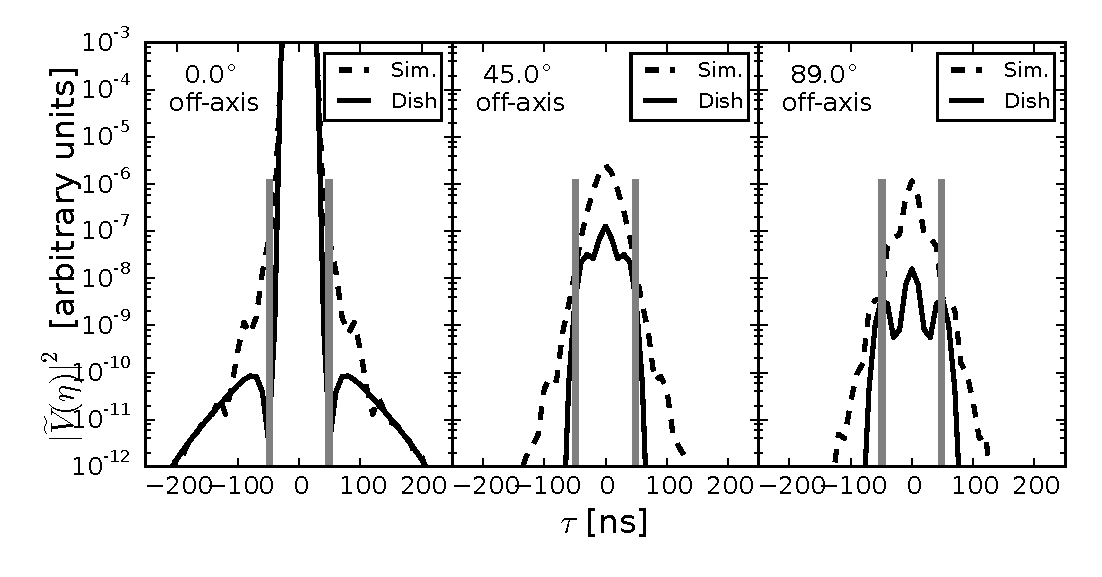
\includegraphics[width=\linewidth]{off-axis_point_source_beam_chromaticity.eps}
\caption{Chromaticity of antenna power pattern at directions off-axis. }
\label{fig:off-axis-beam-chromaticity}
\end{figure*}

At 0\arcdeg off-axis, the {\it Airy} pattern has no spectral variation except that introduced by the {\it Blackman-Harris} window function and thus reproduces its Fourier response centered at $\tau = 0$~ns whereas the simulated power pattern is found to exhibit some spectral variation giving rise to the wings on either side of $\tau = 0$~ns. As off-axis angle increases to 45\arcdeg, both the power patterns clearly exhibit chromaticity. The simulated pattern not only has a higher magnitude inside the horizon limits (by a factor $\sim 10$) but also exhibits higher chromaticity (by many orders of magnitude) in modes beyond the horizon relative to that of an {\it Airy} pattern. In contrast, at 89\arcdeg off-axis, not only does the simulated pattern have higher chromaticity in high delay modes but is also two orders of magnitude higher in amplitude inside the horizon limits relative to the nominal {\it Airy} pattern.

It is important to note that in a generic scenario where visibilities are not phased to a specific foreground location, the chromaticity of the power pattern will imprint itself on location of the foreground objects in delay space and will give rise to significant spillover especially from foregrounds near the horizon. 

We generalize the analysis above by computing the delay power spectrum of the power pattern along its spectral axis in every direction in an effort to study its performance as a function of angle on the sky. 
\begin{align}
  A^\prime(l,m,\tau) &= \int A(l,m,f)\,e^{-j 2\pi f\tau} \,\dif f
\end{align}

We define the directional chromaticity of antenna power pattern as:
\begin{align}
  C(l,m) &= \frac{ \int\limits_{|\tau|>60\,\textrm{ns}} |A^\prime|^2 \,\dif\tau }{\int\limits_{|\tau|>60\,\textrm{ns}} \dif\tau}
\end{align}
where, the limit $|\tau|>60$~ns was chosen to represent a region well beyond the horizon limits ($\pm 48.7$~ns) for a 14.6~m antenna spacing. It thus measures the average power arising out of chromaticity in each delay mode beyond $|\tau|>60$~ns. 

Fig.~\ref{fig:directional-beam-chromaticity} shows the directional chromaticity, $C(l,m)$, of the power patterns of an {\it Airy} disk for reference (left) and a simulated disk (middle) on an orthographic projection onto direction cosines. Their color scale is shown at the top for reference. The chromaticity of the {\it Airy} pattern is symmetric and always below 500. On the other hand,  a simulated disk exhibits higher levels of chromaticity in the range 100--50,000. The ratio of their chromaticities is shown on the right with corresponding color scale on its right. The simulated disk is more chromatic than the nominal {\it Airy} disk by a factor between 100 and up to 10000. However, chromaticity in regions near the horizon which map to the horizon limits in the delay spectrum and have the most significant impact on spillover into the {\it EoR window} in the simulated disk are higher than that of an {\it Airy} disk only by factors $\lesssim 4$. Thus the simulated disk for HERA achieves reasonable control on the chromaticity near the horizon despite the very high levels near the center. 

Also shown are the tracks (black dots) of point sources brighter than 50~Jy in the LST range 0--12~hrs. The solid circle near the bottom denotes the south celestial pole. It is noted that there are a few bright point sources that spend a majority of time in this LST range near the northern and southern horizons which will contaminate the measured visibilities on north-south antenna spacings. Simulations of the antenna power pattern must take the bright foreground locations, especially near the horizon, into account.

\begin{figure*}[htb]
\centering
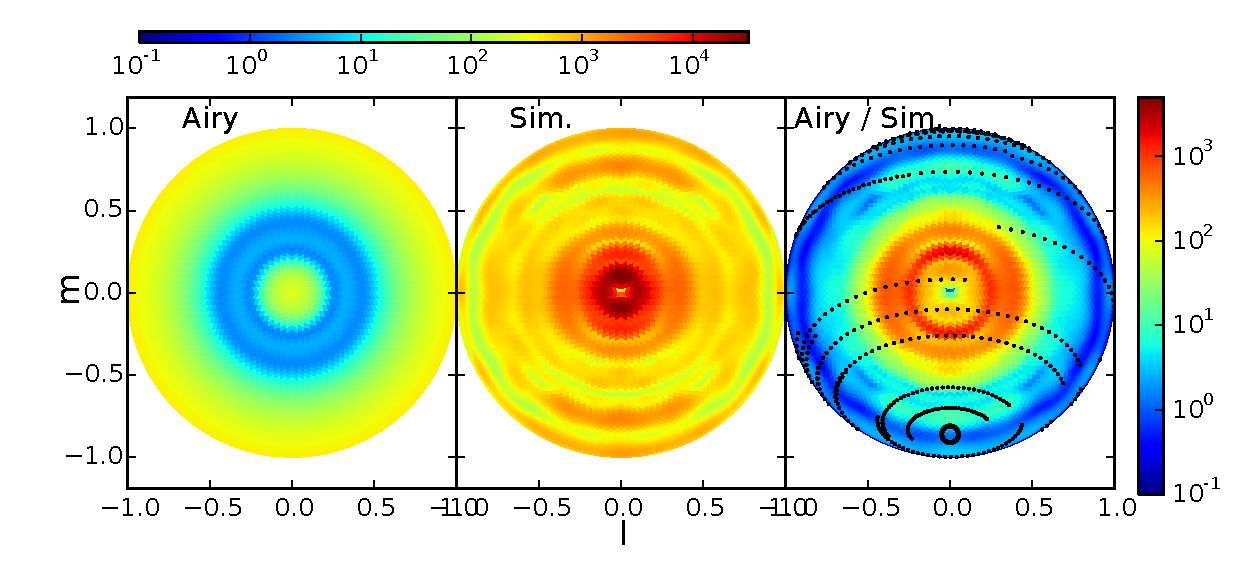
\includegraphics[width=\linewidth]{directional_high_delay_average_in_beam.eps}
\caption{All-sky directional chromaticity of antenna power pattern. }
\label{fig:directional-beam-chromaticity}
\end{figure*}

\subsection{Effect on Delay Power Spectrum}\label{sec:chromaticity-delay-spectrum}

Now we consider the effect of chromaticity of the power pattern on the delay power spectrum. 

In HERA-19 array layout configuration, there are 30 unique baseline vectors and 8 unique baseline lengths. Fig.~\ref{fig:asm-dps-beam-chromaticity-baselines} shows the delay power spectra of foregrounds on the 8 unique baseline lengths obtained with the aforementioned models for power pattern. In all these panels, the full-band foreground delay power spectra obtained with achromatic, {\it Airy} and chromatic beam patterns are shown in black, red, and blue respectively. The vertical dotted lines denote the horizon limits for baseline lengths indicated in each panel. A clear trend of broadening of spillover-wings outside the horizon limits is seen with increasing chromaticity. For instance, the spillover from foreground delay power spectrum obtained with chromatic beam pattern is restricted to $|k_\parallel| \lesssim 0.2\,h$~Mpc$^{-1}$, with the {\it Airy} pattern it is restricted to $|k_\parallel| \lesssim 0.15\,h$~Mpc$^{-1}$, while with the achromatic beam it is restricted to $|k_\parallel| \lesssim 0.12\,h$~Mpc$^{-1}$ even on longest baseline lengths. Thus an increase in chromaticity extends the foreground spillover into higher $k_\parallel$-modes making them inaccessible for EoR H{\sc i} signal detection.

Hence it is clearly demonstrated that higher the beam chromaticity, the farther the foreground contamination inherently extends beyond the horizon limits of the {\it foreground wedge}. The {\it Airy} pattern typically creates one secondary peak whereas the chromatic beam is found to produce multiple secondary peaks outside the {\it foreground wedge} on each side.

\begin{figure*}[htb]
\centering
\includegraphics[width=\linewidth]{asm_foreground_eor_beam_chromaticity_fullband.eps}
\caption{Effect of chromaticity of antenna power pattern on foreground delay power spectra for different baselines.}
\label{fig:asm-dps-beam-chromaticity-baselines}
\end{figure*}

It must be emphasized that such a significant spillover is not limited by the horizon limits of the {\it foreground wedge} because this is caused by spectral structure in the antenna beam pattern in addition to that caused by position-dependent geometric phase in the visibility spectra. As a result delay-based complex deconvolution techniques such as CLEAN \citep{tay99,par09,par12b} that rely on smoothness of foreground spectra and only spectral window shape will not have adequate information to accurately deconvolve intrinsic supra-horizon spillover arising from the chromaticity of the antenna beam. Thus, we leave delay power spectrum estimation using {\it foreground removal} strategy to future work and use {\it foreground avoidance} approach in this study.

We investigate the effect of chromaticity of power pattern in a {\it foreground avoidance} strategy that avoids the aforementioned deconvolution of delay spectrum. Application of window functions with high sidelobe suppression have been discussed for mitigating foreground contamination \citep{thy13}. In line with the {\it foreground avoidance} strategy, Fig.~\ref{fig:asm-dps-beam-chromaticity-baselines-150-subband} shows delay spectra after applying a {\it Blackman-Harris} window function extending 10~MHz on each side centered on 150~MHz with effective bandwidth of 10~MHz. The 8 panels correspond to those shown in Fig.~\ref{fig:asm-dps-beam-chromaticity-baselines}. As a result of narrowed subband, the resolution in delay space (and $k_\parallel$) has coarsened. The cyan and gray lines denote power spectra of EoR models 1 and 2 respectively. 

\begin{figure*}[htb]
\centering
\includegraphics[width=\linewidth]{sim_asm_foreground_eor_beam_chromaticity_150.0_MHz_subband.eps}
\caption{Effect of chromaticity of antenna power pattern on foreground delay power spectra obtained from the 150~MHz subband for different baseline lengths.}
\label{fig:asm-dps-beam-chromaticity-baselines-150-subband}
\end{figure*}

Firstly, it is noted that the coarsening of delay resolution significantly absorbs the distinct differences caused by beams of different chromaticities as seen in the full band foreground delay spectra outside the {\it foreground wedge} in Fig.~\ref{fig:asm-dps-beam-chromaticity-baselines}. Secondly, it is also found that barring the shortest baselines ($|\boldsymbol{b}| \leq $~29.2~m), which have the most severe foreground contamination especially from diffuse emission, foreground contamination on baselines longer than $\gtrsim 29.2$~m is lesser than EoR signal power for $|k_\parallel| \gtrsim 0.22\,h$~Mpc$^{-1}$ in either of the models. 

Fig.~\ref{fig:asm-dps-beam-chromaticity-baselines-170-subband} is similar to Fig.~\ref{fig:asm-dps-beam-chromaticity-baselines-150-subband} except it is obtained with a subband {\it Blackman-Harris} window function centered on 170~MHz. In this subband relative to that centered on 150~MHz, the ratio of powers of the EoR signal and foregrounds is even higher outside the wedge thus indicating a stronger potential for direct detectability without the use of optimal power spectrum estimation techniques on almost all baseline lengths. 

\begin{figure*}[htb]
\centering
\includegraphics[width=\linewidth]{sim_asm_foreground_eor_beam_chromaticity_170.0_MHz_subband.eps}
\caption{Effect of chromaticity of antenna power pattern on foreground delay power spectra obtained from the 170~MHz subband for different baseline lengths.}
\label{fig:asm-dps-beam-chromaticity-baselines-170-subband}
\end{figure*}

It must be emphasized that these are obtained only with windowing techniques and do not represent the best sensitivity achievable with sophisticated tools such as optimal covariance-based weighting schemes \citep{liu14a,liu14b,ali15,dil15}. Thus assuming the data is limited by foregrounds and not by thermal noise, this demonstrates that even with no sophistication in power spectrum estimation, a direct detection based on simple windowing and delay spectrum technique is possible on a majority of HERA baselines and will further allow distinguishing between different EoR models. This finding holds even in the most conservative scenario where the modeled beam pattern with most severe chromaticity inherently results in significant and inherent foreground contamination outside the {\it foreground wedge}.

% Owing to the chromaticity of power patterns, the spillover from foregrounds extends beyond the horizon limits, most severely in the simulated disk pattern. As a result the residuals have significant power remaining on either side of the horizon limits since the window for deconvolution is narrower than the extent of spillover along $k_\parallel$. The two peaks on either side is most severe for the simulated disk pattern followed by that for the {\it Airy} disk pattern and least for an achromatic power pattern. 

% We investigate the effect of chromaticity of power pattern in a foreground avoidance strategy that avoids the aforementioned deconvolution of delay spectrum. Application of window functions with high sidelobe suppression have been discussed for mitigating foreground contamination \citep{thy13}. In line with the foreground avoidance strategy, the visibilities from the full band foreground simulation (whose delay power spectrum is shown on the top left) are multiplied by a Blackman-Harris window function of 10~MHz effective bandwidth. The delay power spectra so produced are shown in the panel on the bottom left. Due to the decreased effective bandwidth the resolution of the delay power spectrum appears decreased. Hence, only the $|k_\parallel| \gtrsim 0.14\,h$~Mpc$^{-1}$ modes remain accessible. Due to the overall lower amplitude of the {\it Airy} power pattern relative to the simulated dish power pattern and the achromatic pattern, the sidelobe levels of foreground delay power spectra from an {\it Airy} pattern are lower than the other models by almost two orders of magnitude. 

% Following a delay-deconvolution based foreground removal strategy, we apply the Blackman-Harris window of effective bandwidth 10~MHz on the unsubtracted foreground residuals (top right panel) in frequency domain and obtain the delay power spectrum shown in the bottom right panel. It is noted that lesser the chromaticity the more effective the deconvolution process is in lowering the residuals in and around the horizon limits. For instance, the peak of the delay power spectrum using the achromatic beam is lowered by four orders of magnitude relative to the original peak whereas the residuals of delay power spectra with chromatic {\it Airy} and simulated power patterns is lowered only by two orders of magnitude. However, owing to the ineffective subtraction of the response extended beyond the horizon limits, the sidelobe levels have not been lowered significantly and are within an order of magnitude of each other.

% In both strategies, the EoR H{\sc i} signal power spectrum obtained by simulations with 21cmFAST (Mesinger et al. 2008) is shown for reference (dashed black lines) in the bottom panels. 

\subsection{Constraints on Reflections between Antennas}\label{sec:reflectometry}

Patra~et~al.~2015 (submitted) and Ewall-Wice~et~al.~2015 (submitted) discuss the measured and simulated reflections between a dish and its feed. We provide a related discussion by estimating the attenuation in power required to keep the foreground power reflected between adjacent antennas below the expected EoR H{\sc i} signal level for the different models of power patterns used in our study.

The effect of reflections it to shift the measured foreground power to higher modes in $\tau$ (or equivalently in $k_\parallel$) and thus cause further contamination in these higher $k_\parallel$ modes which are considered sensitive for EoR H{\sc i} signal detection. Here we estimate the attenuation required at specific $k_\parallel$ modes of interest to contain reflected foreground power between antennas below expected EoR H{\sc i} power, both corresponding to a 14.6~m antenna spacing. 

We define the required attenuation as the ratio: 
\begin{align}
  \Gamma_{k_\parallel}(\tau) &= \frac{P_\textrm{H{\sc i}}(k_\parallel)}{P_\textrm{FG}(k_\parallel - \frac{\dif k_\parallel}{\dif \tau}\,\tau)},
\end{align}
where, $P_\textrm{H{\sc i}}(k_\parallel)$ is the EoR H{\sc i} power spectrum for the chosen antenna spacing, $P_\textrm{FG}(k_\parallel)$ is the foreground delay power spectrum obtained with a Blackman-Harris window function applied over the full band of the three uniquely oriented 14.6~m antenna spacings further averaged over a 0--12 hr LST range and over both positive and negative $k_\parallel$ modes, $\tau$ is the delay caused by reflections, and $\dif k_\parallel/\dif \tau$ is the {\it jacobian} in the transformation of $\tau$ to $k_\parallel$. 

Fig.~\ref{fig:fg-reflections} shows $\Gamma_{k_\parallel}(\tau)$ (in dB) for selected $k_\parallel$ at 0.08~$h$~Mpc$^{-1}$ (left), 0.1~$h$~Mpc$^{-1}$ (middle), and 0.12~$h$~Mpc$^{-1}$ (right) as a function of delays due to reflections from other antenna spacings. The light, medium and dark shaded curves show $\Gamma_{k_\parallel}(\tau)$ for achromatic, {\it Airy}, and chromatic antenna power patterns respectively. These curves set an upper limit to the reflected foreground power below the EoR H{\sc i} signal power as a function of delays caused by antenna-to-antenna reflections. It is noted that a chromatic simulated power pattern sets the most severe upper limit in all three chosen $k_\parallel$ for delays $\tau < 80$~ns (left), $\tau < 120$~ns (middle), and $\tau < 160$~ns. 

\begin{figure*}[htb]
\centering
\includegraphics[width=\linewidth]{spec_on_foreground_reflected_power_21cmfast_14.6m_150.0_MHz_subband_v2.eps}
\caption{Attenuation of foreground power (in dB) from antenna-to-antenna reflections required to keep the reflected foreground power below EoR H{\sc i} signal power.}
\label{fig:fg-reflections}
\end{figure*}

The required attenuation is also a sensitive function of the chosen $k_\parallel$ mode. For instance, at $k_\parallel=0.08\,h$~Mpc$^{-1}$, the reflections with delays 70~ns require to be attenuated by at $\gtrsim 85$~dB for the simulated power pattern, $\gtrsim 82$~dB for the {\it Airy} pattern, and $\gtrsim 70$~dB for the achromatic pattern. However, at $k_\parallel=0.1\,h$~Mpc$^{-1}$ for the same delay of reflection, the requirement on attenuation is lowered to $\gtrsim 75$~dB, $\gtrsim 30$~dB and $\gtrsim 22$~dB respectively. If the chosen $k_\parallel$ is instead 0.12~$h$~Mpc$^{-1}$, the required attenuation is further relaxed to $\gtrsim 60$~dB, $\gtrsim 15$~dB and $\gtrsim 15$~dB respectively. This further reinforces the significance of reducing the chromaticity of the antenna power pattern to further relax the constraint on the system to achieve the attenuation required to contain the reflected foreground power from other antennas from contaminating the sensitive EoR H{\sc i} signal modes in the {\it EoR window}.

\section{Summary}\label{sec:summary}

\acknowledgments

This work was supported by the U. S. National Science Foundation (NSF) through award AST-1109257. DCJ is supported by an NSF Astronomy and Astrophysics Postdoctoral Fellowship under award AST-1401708. JCP is supported by an NSF Astronomy and Astrophysics Fellowship under award AST-1302774. 

% \appendix

% \par\bigskip
\bibliographystyle{apj}
\bibliography{eor}

\end{document}
